\documentclass[11pt]{article}
\usepackage[margin=1in]{geometry}
\usepackage[T1]{fontenc}
\usepackage[utf8]{inputenc}
\usepackage{amsmath,amssymb}
\usepackage{fancyhdr}
\usepackage{graphicx}
\usepackage[table]{xcolor}
\setlength{\intextsep}{4pt}

\pagestyle{fancy}
\fancyhf{}
\fancyhead[L]{Cristian Bautista}
\fancyhead[C]{CSE 5525 -- Assignment 2}
\fancyhead[R]{\today}
\fancyfoot[C]{\thepage}
\setlength{\headheight}{15pt}
\renewcommand{\headrulewidth}{0.4pt}
\renewcommand{\footrulewidth}{0.4pt}

\begin{document}
\section*{Deep Averaging Network Sentiment Classification}

\noindent\textbf{Implementation.}
A deep averaging network (DAN) was implemented in PyTorch, first processing
one sentence per update. A length-$L$ sentence becomes
indices $(L,)$ and frozen GloVe embeddings $(L,300)$. Averaging across words
gives a fixed-size vector $(300,)$.
The network applies a $300\!\to\!100$ linear layer, ReLU, a $100\!\to\!2$
linear layer, and LogSoftmax. Its two log-probabilities represent negative
and positive sentiment, prediction selects their argmax. Linear weights
use Xavier initialization, and Adam minimizes negative log-likelihood.

\smallskip
\noindent\textbf{Exploration: batching and padding.}
Groups of $B$ sentences are padded to their maximum length $L_{\max}$ with
\texttt{PAD} (index 0), giving indices $(B,L_{\max})$ and embeddings
$(B,L_{\max},300)$. A Boolean mask $M_{bj}=\mathbf{1}[x_{bj}\ne0]$ counts
real tokens, $n_b=\sum_j M_{bj}$ and determin the length of the sentence. Frozen PAD vectors are zero, so embeddings
can be summed directly: $\bar e_b=\sum_j e(x_{bj})/n_b$.
Dividing sums $(B,300)$ by real lengths $(B,1)$ excludes padding from the
average; UNK still counts as a word. Hidden activations are $(B,100)$ and
outputs $(B,2)$, with LogSoftmax over the class axis. Labels are $(B,)$;
\texttt{NLLLoss} averages their losses for one backward pass and update per
batch, including the final smaller group. Evaluation processes each
sentence as $(1,L)$ and selects its sole output row.

\smallskip
\noindent\textbf{Experimental setup.}
Batch sizes 1, 16, and 32 were trained for ten epochs on 6,920 examples,
with learning rate 0.001, hidden size 100, and seed 42, shuffling each epoch.
Train and dev (872 examples) mean loss and accuracy are evaluated after
each epoch with fixed weights and disabled gradients. Best dev accuracy is
recorded, but the returned model retains the final epoch's weights. The training was done using \texttt{torch-cpu} in a Intel Ultra 9 285H.

% Generated by p2-distrib/plot_history.py from the selected metric CSVs.
\begin{table}[!ht]
\centering
\small
\caption{DAN batching over 10 epochs (seed 42). Best epoch maximizes dev accuracy; final dev uses the last epoch. Training time excludes evaluation. Speedups are relative to batch size 1 and use one run per configuration.}
\label{tab:batch-results}
\setlength{\tabcolsep}{4pt}
\renewcommand{\arraystretch}{1.1}
\begin{tabular}{rrrrrr}
\hline
Batch & Best dev (\%) & Epoch & Final dev (\%) & Train (s) & Speedup \\
\hline
1 & 78.33 & 2 & 77.18 & 125.01 & 1.00$\times$ \\
16 & \cellcolor{gray!20}\textbf{78.90} & 3 & 78.44 & 5.14 & 24.30$\times$ \\
32 & 78.78 & 7 & 78.56 & 2.80 & 44.66$\times$ \\
\hline
\end{tabular}
\end{table}


\noindent\textbf{Results and discussion.}
Batch 16 achieved the best observed dev accuracy, 78.90\% at epoch 3
(Table~\ref{tab:batch-results}), one more correct prediction than batch 32
at its best epoch (688 versus 687 of 872). Batch 32 had the highest final
dev accuracy, 78.56\%; all final models exceeded 77\% (Figure~\ref{fig:dev-accuracy}).
For batch 1, train loss fell from 0.452 to 0.280, but dev loss increased
from its epoch-2 minimum of 0.452 to 0.520 (Figure~\ref{fig:loss}).
Its final train/dev accuracy gap was 10.29 percentage points, versus 7.27
and 5.95 for batches 16 and 32, whose final dev losses were 0.456 and 0.462.
These results suggest less overfitting with the larger batches in these runs.
Loss also reflects confidence: batch 16 minimized dev loss at epoch 2,
but maximized accuracy at epoch 3.

Training times were 125.01, 5.14, and 2.80 seconds, respectively:
measured speedups of $24.30\times$ and $44.66\times$, including batch
preparation but excluding evaluation. Equal epochs
therefore expose models to the same examples but give different update
counts and optimization trajectories. Larger batches were faster and had
better final dev accuracy here; small accuracy differences and single-seed,
single-run timings limit broader conclusions about batch size.

Future work could explore fine-tuning the pretrained word embeddings and
varying the number of hidden layers. Given the observed train--dev gap,
dropout could be evaluated to reduce overfitting. Alternative aggregation
strategies, such as max pooling, could also be compared with the current
averaging operation. Finally, architectures such as
LSTMs, could capture word order, which the DAN discards.


\clearpage
\begin{figure}[!ht]
\centering
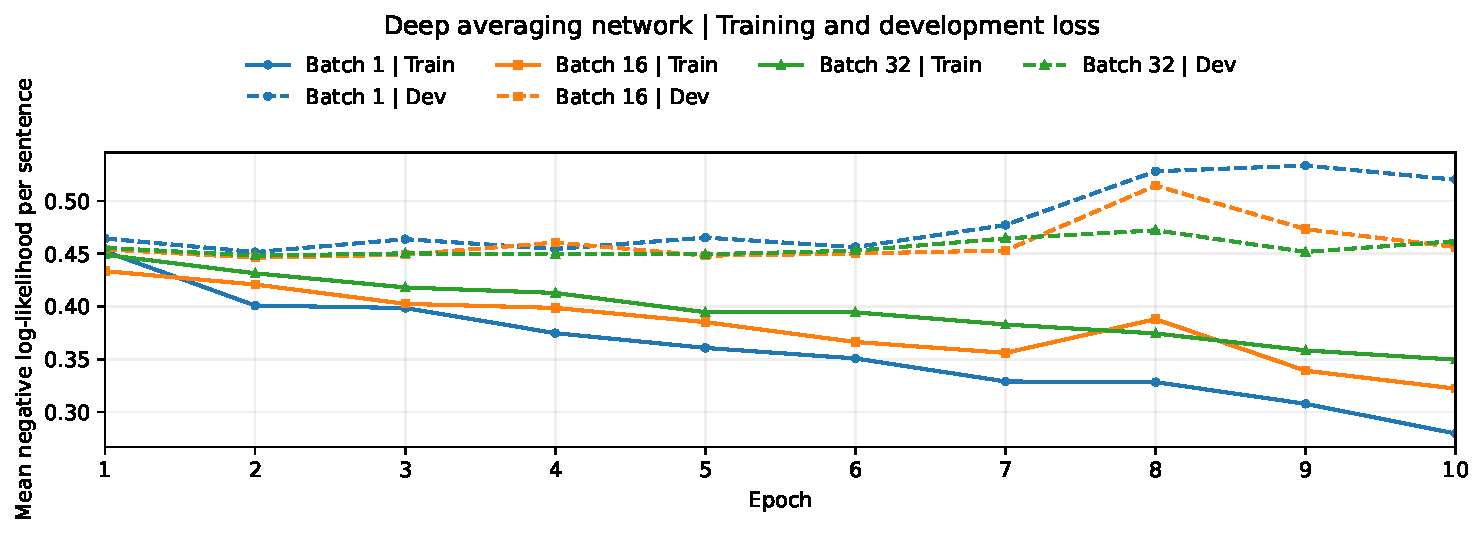
\includegraphics[width=\textwidth]{figures/loss_comparison.pdf}
\small
\caption{Mean training and development negative log-likelihood per sentence
over ten epochs for batch sizes 1, 16, and 32. Solid curves show training
loss and dashed curves show development loss. Both sets are evaluated
using the weights at the end of each epoch; padding is excluded from
the sentence averages.}
\label{fig:loss}
\end{figure}

\begin{figure}[!ht]
\centering
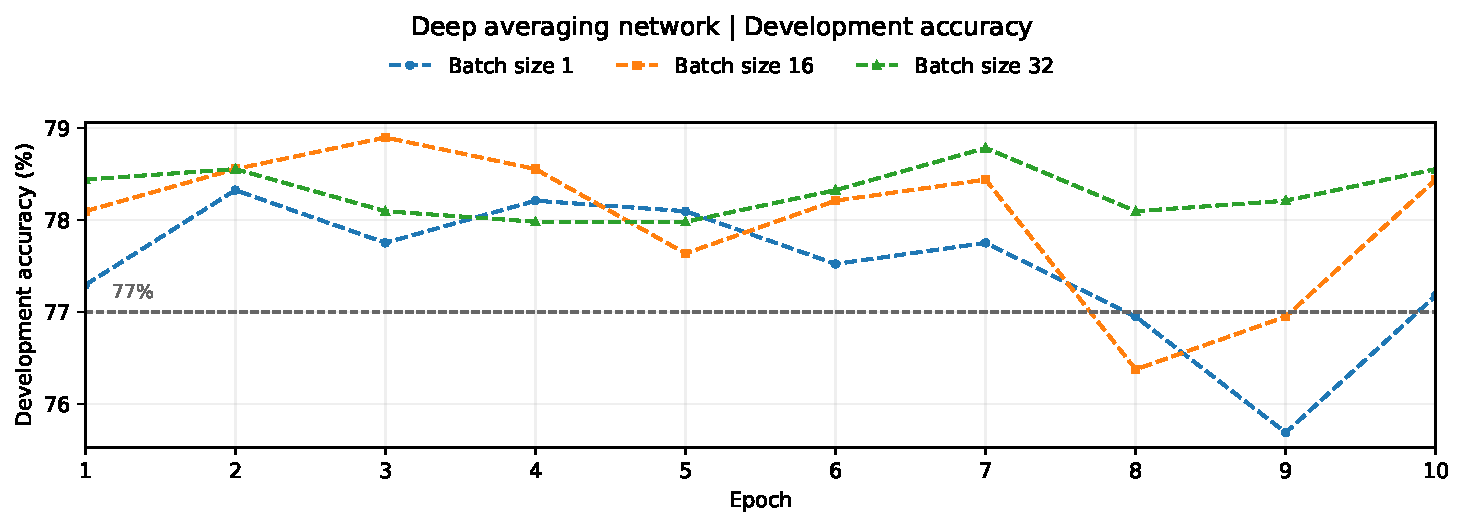
\includegraphics[width=\textwidth]{figures/dev_accuracy_comparison.pdf}
\small
\caption{Dev accuracy over ten epochs for batch sizes 1, 16,
and 32, using seed 42. The horizontal gray dashed line marks the
77\% accuracy target. Each curve uses the corresponding complete
ten-epoch experiment reported in Table~\ref{tab:batch-results}.}
\label{fig:dev-accuracy}
\end{figure}
\end{document}
